
\section{Objectifs}
\paragraph{}
Lorsque l'on prouve des théorèmes, on a souvent l'impression de faire la même chose, on obtient des reflexes dans de nombreuses situations. Dans les domaines les plus utilisés, il existe maintenant des tactiques résolvant ces opérations répétitives (auto de manière générale, omega pour les entiers naturels, field dans les corps,...).

\paragraph{}
Cependant, lorsque l'on travaille sur des outils plus rares, ou des outils que l'on a soit-même défini, il n'existe pas de tactiques prédéfinies. 

\paragraph{}
Une solution serait de construire soit-même ses propres tactiques lorsque l'on définit de nouveau concept. Malheureusement, celà est difficile. D'une part, parce que Ltac est assez difficile à maîtriser, d'autre part parce qu'il est difficile de transformer un savoir-faire composé de reflexes en une description de ce savoir-faire.

\paragraph{}
L'objectif de ce groupe de travail est de remédier à ce problème. On cherche donc à créer automatiquement, à partir de nombreuses démonstrations, des tactiques permettant de faire des démonstrations similaires.

\section{Les arbres de décisions}

\paragraph{Pourquoi des arbres de décision}
Après une revue des méthodes classiques d'apprentissage, nous avons résolu des théorèmes en coq en analysant à chaque étape notre raisonnement. Nous avons remarqué que nous réflechissions le plus souvent comme des arbres de décision. Nous nous interrogeons sur la structure des hypothèses et du but, à commencer par les noeuds de l'arbre syntaxique de moindre profondeur. La racine du but nous donne assez souvent, à elle seule, la tactique à utiliser. La plupart du temps, si le but est ``T\&U'' on utilise ``split'', si le but est ``forall x, T'' ou ``T -> U'' on utilise intro.  

\paragraph{Définition des arbres de décision}
Un arbre de décision est défini par induction comme étant :
\begin{itemize}
\item Une liste de réponse
\item Une question sur la situation, et pour chaque valeur un arbre de décision
\end{itemize}

\paragraph{Possibilités pour les questions}
D'après ce que nous avons dit plus haut, il est logique de poser les questions sur le haut des arbres. Donc on s'autorise à interroger le noeud à la racine des arbres syntaxiques des hypothèses et du but, ainsi que les fils des arbres déjà interrogés. Les questions qu'on leur pose sont What addr (quel est le token à l'addresse addr?) et Equal addr1 addr2 (est-ce que les tokens à l'addresse addr1 et à l'addresse addr2 sont les même?).


\paragraph{Exemple}
Ici, si le but est de la forme T=T, on répondra $reflexivity$. Son(i,j) désigne le j-ième fils de l'arbre interrogé à la profondeur i.

\paragraph{}
Si la valeur ne correspond à aucune autre, on prend la branche $\$\$OTHER\$\$$
\begin{figure}[h]
  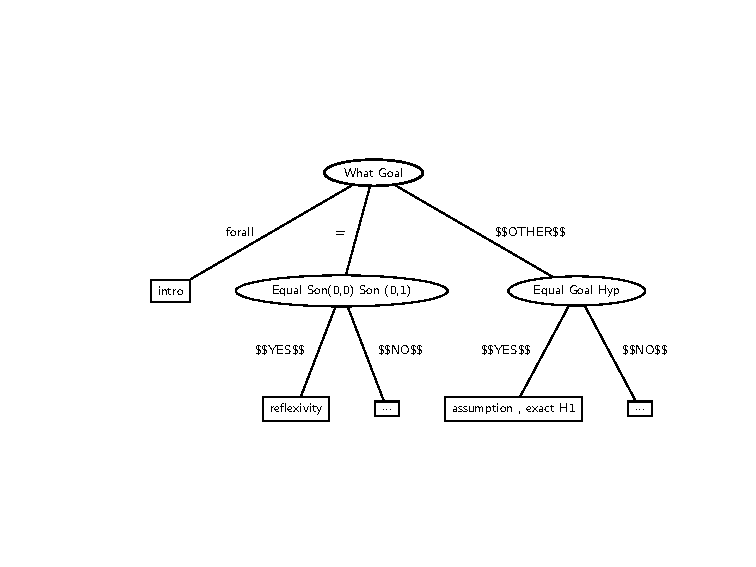
\includegraphics[scale=1.7]{../images/apprentissage/decision_tree.jpg}
\end{figure}


\section{Organisation des modules}
  \begin{figure}[h]
    \includegraphics[scale=0.35]{../images/apprentissage/organisation_apprentissage.pdf}
  \end{figure}
  \subsection{Fouille sur net/résolution d'exos}
  Un premier travail est de rassembler un grand nombre de démonstration dans un même domaine. Nous nous sommes essayé sur deux domaines : la logique du premier ordre et les comparaisons d'entiers. Pour des tactiques complète pour ces domaines, il faudrait plus de lignes de démonstrations. Mais ces collections suffisent à tester notre algorithme.
  \subsection{Parsing, discussion avec coqtop}
  Les fichiers que l'on récolte sont des fichiers coqs normaux. Il faut ensuite en extraire les exemples que l'on va apprendre. Il faut donc dialoguer avec coqtop pour qu'à chaque ligne de chaque démonstration on récupère les hypothèses et le but courant. On récupère également la tactique que le mathématicien a utilisé dans cette situation. Les tactiques ne sont pas considérées comme des simples chaînes, on repère lorsqu'elles prennent en argument une hypothèse de l'environnement. On transforme tout ça dans la forme dont a besoin l'algorithme d'apprentissage.

  \subsection{Algorithme d'apprentissage} 
  L'algorithme d'apprentissage transforme ces données experimentales en un arbre de décision (cf la section correspondante).

  \subsection{Traduction}
  L'arbre est transformé automatiquement en une tactique, qui pourra ensuite être utilisée telle quelle.


\section{Apprentissage}
\subsection{Entropie}
On considère un ensemble $\{x_i\}_{i \in I}$. On tire au hasard $n$ fois un $x_i$ ($x_j$ est pris avec la probabilité $p_j$). Le meilleur code décrivant la suite des éléments tirés a une espérance de longueur de $n * \sum_{i \in I}{- p_i * \log{p_i}}$. On définit alors \strong{l'entropie} du tirage comme $ \sum_{i \in I}{- p_i * \log{p_i}}$, soit environ la longueur moyenne du code décrivant quel élément a été tiré. En particulier, on remarque que si une seule réponse est possible l'entropie est nulle.

\subsection{Application de l'entropie aux arbres de décision}
Nous voulons qu'à chaque feuille de l'arbre de décision, l'entropie soit minimale. C'est à dire que, pour les exemples conduisant à une même feuille, la tactique à utiliser soit toujours la même. Il faut donc diminuer l'entropie à chaque étape. On veut que l'arbre soit de taille minimale, donc il faut maximiser la perte d'entropie moyenne sur le nombre de noeud total de l'arbre de décision.\\

La maximisation exacte n'est (a priori) même pas dans NP. Il paraît donc préferable d'utiliser une heuristique. A chaque noeud de l'arbre de décision, on cherche à maximiser la perte d'entropie sur le nombre de fils. Pour celà, pour toute les questions possibles, on mesure l'entropie moyenne après la question.


\section{Transformation en tactique}

\section{Difficultés surmontées}

\section{Pipeau?}

\section{Résultats}
Le parcours d'arbres et le rafinement des données sont utilisables (leur complexité est améliorable et des améliorations sont possibles).
 L'algorithme d'apprentissage a été réalisé, il faut maintenant le tester pour vérifier qu'il correspond bien à nos attentes.

\section{Améliorations futures}
